\chapter{K3 Surfaces: Definition, Examples and Topology}\label{ch:k3}

Up to this point the compact spaces of this book were tori. A torus is flat, its string spectrum
can be written in closed form, and its duality group $\Odd{d}$ acts on an explicit lattice of
momenta and windings (\cref{ch:narain,ch:odd}). The price is that a flat space has trivial
holonomy and therefore breaks no supersymmetry at all. The next simplest compact space on which a
string can propagate consistently is curved, and in real dimension four there is essentially one
choice: the K3 surface\index{K3 surface}. This chapter answers three questions. What is a K3
surface, and how does one write one down? What are its topological invariants, in particular
the numbers $24$, $22$, $20$ and $(3,19)$ that will reappear in every later chapter of Part~IV?
And why do physicists care: what is special about the holonomy of a K3 surface, and what does it
do to supersymmetry? The reader needs no algebraic geometry beyond what is recalled here; the
two tools we use repeatedly are Chern classes, treated as formal polynomials, and the
Riemann--Roch formula, treated as a black box with a precise statement. The lattice that the
invariants determine, $3U\oplus 2E_8(-1)$, was constructed in \cref{ch:lattices} and is studied
as the cohomology of a K3 surface in \cref{ch:k3lattice}.

\section{The definition and what each condition means}\label{sec:k3:def}

Let $X$ be a compact connected complex manifold of complex dimension two, a \emph{complex
surface}. It carries the sheaf $\mathcal{O}_X$ of holomorphic functions, the rank-two bundle
$\Omega_X$ of holomorphic one-forms $a_1\,\dd z_1+a_2\,\dd z_2$, and its top exterior power, the
\emph{canonical bundle}\index{canonical bundle} $\omega_X=\Omega_X^2=\Lambda^2\Omega_X$, whose
local sections are the holomorphic two-forms $a\,\dd z_1\wedge\dd z_2$. Its first Chern class
is $c_1(\omega_X)=-c_1(T_X)$, where $T_X$ is the holomorphic tangent bundle; the class
$K=-c_1(T_X)$ is called the canonical class.

\begin{definition}[K3 surface]\label{def:k3:k3}
A \emph{complex K3 surface} is a compact connected complex manifold $X$ of complex dimension two
such that
\begin{equation}\label{eq:k3:def}
  \Omega_X^2\;\cong\;\mathcal{O}_X
  \qquad\text{and}\qquad
  H^1(X,\mathcal{O}_X)=0 .
\end{equation}
\source{Huy ch.~1, Def.~3.1, ll.~464--465; algebraic version over any field: Def.~1.1,
ll.~158--161}
\end{definition}

Both conditions have a direct meaning.

\paragraph{Trivial canonical bundle.} The isomorphism $\Omega_X^2\cong\mathcal{O}_X$ says that
there is a holomorphic two-form $\Omega$ on $X$ that vanishes nowhere. It is unique up to a
constant: if $\Omega'$ is a second one, the ratio $\Omega'/\Omega$ is a holomorphic function on a
compact connected manifold, hence constant by the maximum principle. So
\begin{equation}\label{eq:k3:h20}
  h^{2,0}(X):=\dim H^0(X,\Omega^2_X)=1 .
\end{equation}
\source{Asp §2.1, ll.~260--265} In particular $c_1(T_X)=0$. The form $\Omega$ also gives a
pairing $\Omega_X\times\Omega_X\to\omega_X\cong\mathcal{O}_X$, $(\alpha,\beta)\mapsto
\alpha\wedge\beta/\Omega$, which is alternating and non-degenerate at every point: a
\emph{holomorphic symplectic structure}\index{holomorphic symplectic form}. It identifies the
tangent bundle with the cotangent bundle, $T_X\cong\Omega_X$ \source{Huy ch.~1 §1,
ll.~165--170}; we use this identification in \cref{sec:k3:hodge}.

\paragraph{No holomorphic one-forms, no first cohomology.} The second condition excludes the
other compact surfaces with a nowhere-vanishing holomorphic two-form, the complex tori
$\C^2/\Gamma$: on a torus $\dd z_1\wedge\dd z_2$ trivializes the canonical bundle, but
$H^1(\mathcal{O})$ is two-dimensional. We will see in \cref{sec:k3:hodge} that
$H^1(X,\mathcal{O}_X)=0$ forces $H^1(X,\Z)=0$, so the first Betti number of a K3 surface
vanishes; in fact a K3 surface is simply connected (\cref{thm:k3:diffeo} below).

\begin{remark}[Two definitions in use]\label{rem:k3:twodefs}
Physics texts often define a K3 surface as a compact complex \emph{Kähler} surface with
$h^{1,0}=0$ and $K=0$ \source{Asp §2.1, ll.~229--233}. The Kähler condition\index{Kähler
manifold} need not be imposed: every complex K3 surface in the sense of
\cref{def:k3:k3} is Kähler, a fact that is ``of great importance, but not easy to prove''
\source{Huy ch.~1 §3.1, ll.~495--497}. \TL{} On a Kähler manifold $h^{1,0}=h^{0,1}$, so the two
definitions agree. Not every complex K3 surface is projective, however; the algebraic ones form
a proper subset \source{Huy ch.~1 §3.1, ll.~486--493}.
\end{remark}

\begin{historybox}[Why ``K3''?]
The name was coined shortly after the first ascent, in 1954, of the mountain K2 in the
Karakoram; it is explained as honouring Kummer, Kähler and Kodaira, with an allusion to that
mountain. It does not mean ``Kummer's third surface'', a reading that circulates in
part of the physics literature. \source{Asp §2, ll.~198--211 and footnote~1, ll.~237--241}
\end{historybox}

The fact that makes the subject tractable is that the definition, which constrains only
holomorphic data, pins down the underlying smooth manifold completely.

\begin{theorem}[One diffeomorphism type]\label{thm:k3:diffeo}
Any two complex K3 surfaces are diffeomorphic. In particular every K3 surface is diffeomorphic
to a smooth quartic in $\mathbb{P}^3$, and is simply connected. \TL{}
\source{Asp §2.1, Theorem~1, l.~236; Huy ch.~1, Remark~3.6(i), ll.~626--632}
\end{theorem}

Consequently \emph{all topological invariants of a K3 surface can be computed on one example}.
This is the strategy of Aspinwall's lectures, followed in \cref{sec:k3:quartic}. Huybrechts
instead derives the same numbers from the definition alone by Riemann--Roch; we do this in
\cref{sec:k3:hodge}. The agreement of the two routes checks every number in this chapter.

\begin{pitfallbox}[``The'' K3 surface]
Physicists say ``the K3 surface'' because of \cref{thm:k3:diffeo}: there is one smooth
four-manifold. As \emph{complex} manifolds K3 surfaces come in a continuous family with
twenty complex parameters, and the choice of a Ricci-flat metric adds further parameters
(\cref{ch:k3lattice,ch:stringsk3}). Topological statements ($\chi=24$, signature $(3,19)$) hold for all of them;
statements about curves, Picard groups or symmetries depend on which member of the family is
meant.
\end{pitfallbox}

\section{The first example: a quartic surface}\label{sec:k3:quartic}

Let $f(x_0,x_1,x_2,x_3)$ be a homogeneous polynomial of degree $n$ and
\begin{equation}\label{eq:k3:hypersurface}
  S_n=\{[x_0:x_1:x_2:x_3]\in\mathbb{P}^3 \;:\; f(x)=0\}.
\end{equation}
We assume $S_n$ smooth: the four partial derivatives $\partial f/\partial x_i$ have no common
zero on $S_n$. The standard example is the Fermat surface\index{Fermat quartic}
$f=x_0^n+x_1^n+x_2^n+x_3^n$ \source{Asp §2.1, eq.~(4), ll.~246--250}. We ask for which $n$ the
surface $S_n$ is a K3 surface, and answer the question twice.

\subsection{Writing down the holomorphic two-form}

In the patch $x_0\neq0$ use affine coordinates $y_i=x_i/x_0$ ($i=1,2,3$) and write
$F(y)=f(1,y_1,y_2,y_3)$, with partial derivatives $F_i=\partial F/\partial y_i$. On the surface
$F=0$ we have $\dd F=F_1\dd y_1+F_2\dd y_2+F_3\dd y_3=0$. Wedge this relation with $\dd y_2$:
$F_1\,\dd y_1\wedge\dd y_2=-F_3\,\dd y_3\wedge\dd y_2=F_3\,\dd y_2\wedge\dd y_3$. Doing the same
with $\dd y_1$ one finds that the three expressions
\begin{equation}\label{eq:k3:residue}
  \Omega\;=\;\frac{\dd y_1\wedge\dd y_2}{F_3}
        \;=\;\frac{\dd y_2\wedge\dd y_3}{F_1}
        \;=\;\frac{\dd y_3\wedge\dd y_1}{F_2}
\end{equation}
agree on $S_n$ wherever they are defined \source{Asp §2.1, eq.~(6), ll.~266--293}. Smoothness
says that at each point at least one $F_i$ is nonzero. Where $F_3\neq0$ the implicit function
theorem makes $(y_1,y_2)$ local coordinates on $S_n$, and the first expression is a holomorphic
two-form without zeros; similarly for the other two. Hence $\Omega$ is holomorphic and nowhere
zero on the whole patch $x_0\neq0$. This is the residue\index{residue form} of the meromorphic
three-form $\dd y_1\wedge\dd y_2\wedge\dd y_3/F$ along $F=0$ \source{Huy ch.~1, Example~1.3(i),
eqs.~(1.1)--(1.2), ll.~194--206}.

The question is what happens on the ``hyperplane at infinity'' $x_0=0$. Aspinwall calls the
check ``straightforward but rather tedious''; it takes six lines. In the patch $x_1\neq0$ use
$u_0=x_0/x_1$, $u_2=x_2/x_1$, $u_3=x_3/x_1$ and $G(u)=f(u_0,1,u_2,u_3)$. On the overlap
\begin{equation}
  y_1=\frac1{u_0},\qquad y_2=\frac{u_2}{u_0},\qquad y_3=\frac{u_3}{u_0},
  \qquad F(y)=u_0^{-n}\,G(u),
\end{equation}
the last equality because $f$ is homogeneous of degree $n$. Then
\begin{align}
  \dd y_1\wedge\dd y_2 &= \Big(-\frac{\dd u_0}{u_0^2}\Big)\wedge
      \Big(\frac{\dd u_2}{u_0}-\frac{u_2\,\dd u_0}{u_0^2}\Big)
      = -\frac{\dd u_0\wedge\dd u_2}{u_0^{3}}, \\
  F_3 &= u_0^{-n}\,\frac{\partial G}{\partial u_3}\,\frac{\partial u_3}{\partial y_3}
      = u_0^{\,1-n}\,G_3 ,
\end{align}
where we used $u_3=y_3/y_1$, so $\partial u_3/\partial y_3=1/y_1=u_0$, while $u_0$ and $u_2$
do not depend on $y_3$. Dividing,
\begin{equation}\label{eq:k3:patch}
  \Omega\;=\;-\,u_0^{\,n-4}\;\frac{\dd u_0\wedge\dd u_2}{G_3}.
\end{equation}
The form $\dd u_0\wedge\dd u_2/G_3$ is the analogue of \eqref{eq:k3:residue} in the second
patch, holomorphic and nowhere zero there. So along the curve $u_0=0$ the form $\Omega$ has a
zero of order $n-4$ if $n>4$, a pole of order $4-n$ if $n<4$, and extends to a nowhere-vanishing
holomorphic two-form exactly when
\begin{equation}
  n=4 .
\end{equation}
For $n\neq4$ equation \eqref{eq:k3:patch} is still informative: it says that the canonical
bundle of $S_n$ is $\mathcal{O}(n-4)$ restricted to $S_n$, the adjunction
formula\index{adjunction formula} $\omega_{S}\cong(\omega_{\mathbb{P}^3}\otimes
\mathcal{O}(n))|_S$ with $\omega_{\mathbb{P}^3}=\mathcal{O}(-4)$ \source{Huy ch.~1,
Example~1.3(i), ll.~190--194}.

The second condition of \cref{def:k3:k3} holds for every $n$: from the exact sequence
$0\to\mathcal{O}(-n)\to\mathcal{O}\to\mathcal{O}_{S}\to0$ on $\mathbb{P}^3$ and the vanishing
$H^1(\mathbb{P}^3,\mathcal{O})=H^2(\mathbb{P}^3,\mathcal{O}(-n))=0$ one reads off
$H^1(S,\mathcal{O}_S)=0$ \source{Huy ch.~1, Example~1.3(i), ll.~185--189}. Topologically this is
the Lefschetz hyperplane theorem, which also gives $\pi_1(S)=0$ \source{Asp §2.1, ll.~253--254
and eq.~(13), ll.~364--366}. Therefore:

\begin{proposition}\label{prop:k3:quartic}
A smooth quartic surface in $\mathbb{P}^3$ is a K3 surface. \TL{}
\end{proposition}

\subsection{Chern classes by adjunction}

The same conclusion, and the Euler characteristic as a bonus, follows from a formal
computation. Let $x\in H^2(\mathbb{P}^3,\Z)$ be the class of a hyperplane; $x^3$ integrates to
$1$ over $\mathbb{P}^3$ and $x^4=0$. The total Chern class of projective space is
$c(T_{\mathbb{P}^k})=(1+x)^{k+1}$, and the normal bundle $N_S$ of a degree-$n$ hypersurface is
$\mathcal{O}(n)|_S$ with $c(N_S)=1+nx$. Since $T_{\mathbb{P}^3}|_S=T_S\oplus N_S$ as smooth
bundles and the total Chern class is multiplicative,
\begin{equation}\label{eq:k3:chern}
  c(T_S)=\frac{(1+x)^4}{1+nx}
  =\big(1+4x+6x^2\big)\big(1-nx+n^2x^2\big)+O(x^3)
  =1+(4-n)\,x+(n^2-4n+6)\,x^2 .
\end{equation}
\source{Asp §2.1, eqs.~(7)--(11), ll.~296--337} So $c_1(T_S)=(4-n)x$, which vanishes exactly for
$n=4$, in agreement with \eqref{eq:k3:patch}. The top Chern class integrates to the Euler
characteristic\index{Euler characteristic!of K3}. To integrate over $S$ we integrate over
$\mathbb{P}^3$ after multiplying with the class dual to $S$, which is $nx$:
\begin{equation}\label{eq:k3:chi24}
  \chi(S_n)=\int_{S_n}c_2(T_S)=\int_{\mathbb{P}^3} nx\cdot(n^2-4n+6)\,x^2=n\,(n^2-4n+6),
  \qquad \chi(S_4)=4\cdot6=24 .
\end{equation}
\source{Asp §2.1, eq.~(12), ll.~337--363}

\begin{example}[The surfaces of degree $1$ to $5$]\label{ex:k3:degrees}
Formula \eqref{eq:k3:chern} can be tested on surfaces the reader already knows. Besides $\chi$
we compute two further characteristic numbers, whose meaning is explained in
\cref{sec:k3:hodge,sec:k3:signature}: the holomorphic Euler characteristic
$\chi(\mathcal{O})=(c_1^2+c_2)/12$ and the signature $\sigma=(c_1^2-2c_2)/3$. With
$c_1^2[S_n]=n(4-n)^2$ and $c_2[S_n]=n(n^2-4n+6)$,
\begin{equation}\label{eq:k3:degreeformulas}
  \chi(\mathcal{O}_{S_n})=\frac{n(n^2-6n+11)}{6},\qquad
  \sigma(S_n)=-\frac{n(n-2)(n+2)}{3}.
\end{equation}
All $S_n$ are simply connected, so $b_1=b_3=0$ and $b_2=\chi-2$; the numbers $b_\pm$ of
positive and negative eigenvalues of the intersection form follow from $b_++b_-=b_2$,
$b_+-b_-=\sigma$.
\begin{center}
\begin{tabular}{@{}cccccccl@{}}
\toprule
$n$ & $c_1$ & $\chi$ & $\chi(\mathcal{O})$ & $\sigma$ & $b_2$ & $(b_+,b_-)$ & surface\\
\midrule
1 & $3x$ & 3 & 1 & $1$ & 1 & $(1,0)$ & the plane $\mathbb{P}^2$\\
2 & $2x$ & 4 & 1 & $0$ & 2 & $(1,1)$ & the quadric $\mathbb{P}^1\times\mathbb{P}^1$\\
3 & $x$ & 9 & 1 & $-5$ & 7 & $(1,6)$ & cubic: $\mathbb{P}^2$ blown up in 6 points\\
4 & $0$ & 24 & 2 & $-16$ & 22 & $(3,19)$ & \textbf{K3}\\
5 & $-x$ & 55 & 5 & $-35$ & 53 & $(9,44)$ & quintic surface (general type)\\
\bottomrule
\end{tabular}
\end{center}
The first three rows reproduce known answers: $\chi(\mathbb{P}^2)=3$; the quadric is a product
of two spheres with $\chi=2\cdot2$ and hyperbolic intersection form $U$; blowing up a point
adds one class of self-intersection $-1$, so six blow-ups of $\mathbb{P}^2$ give $\chi=3+6$ and
$(b_+,b_-)=(1,6)$. The row $n=4$ contains every number of this chapter. It is the only row with
$c_1=0$: positive $c_1$ ($n<4$) gives rational surfaces, negative $c_1$ ($n>4$) surfaces of
general type, and K3 sits on the boundary, as a Ricci-flat space should. (The table is a symbolic check with sympy; the identification of the low-degree surfaces is
standard and not checked against a source in this book's library.)
\end{example}

\section{More examples}\label{sec:k3:examples}

The quartic is one member of a short list of classical constructions
\source{Huy ch.~1, Example~1.3, ll.~185--270}. Each gives K3 surfaces depending on parameters,
and by \cref{thm:k3:diffeo} each must have $\chi=24$, which we verify as a check of the method.

\subsection{Complete intersections}\index{complete intersection}

Let $S\subset\mathbb{P}^{m+2}$ be a smooth surface cut out by $m$ homogeneous equations of
degrees $d_1,\dots,d_m$. The normal bundle is $\bigoplus_i\mathcal{O}(d_i)|_S$ and
\eqref{eq:k3:chern} becomes
\begin{equation}\label{eq:k3:ci}
  c(T_S)=\frac{(1+x)^{m+3}}{\prod_{i}(1+d_ix)}
  \quad\Longrightarrow\quad
  c_1(T_S)=\Big(m+3-\sum_i d_i\Big)x .
\end{equation}
So $S$ is a K3 surface if and only if $\sum_id_i=m+3$. A linear equation ($d_i=1$) only lowers
the dimension of the ambient projective space, so assume all $d_i\ge2$; then $2m\le m+3$ leaves
exactly three cases \source{Huy ch.~1, Example~1.3(ii), ll.~212--217}:
\begin{center}
\begin{tabular}{@{}lcccc@{}}
\toprule
ambient space & degrees $(d_i)$ & $c_2(T_S)$ & degree $\prod d_i$ & $\chi=\prod d_i\cdot c_2$\\
\midrule
$\mathbb{P}^3$ & $(4)$ & $6x^2$ & 4 & 24\\
$\mathbb{P}^4$ & $(2,3)$ & $4x^2$ & 6 & 24\\
$\mathbb{P}^5$ & $(2,2,2)$ & $3x^2$ & 8 & 24\\
\bottomrule
\end{tabular}
\end{center}
For instance, for $(2,3)$: $(1+x)^5=1+5x+10x^2$, $1/[(1+2x)(1+3x)]=1-5x+19x^2$, and the $x^2$
coefficient of the product is $10-25+19=4$. The class dual to $S$ is $\prod d_i\,x^m$, which
supplies the factor $6$. The three Euler characteristics agree, as they must. (The
$c_2$ column and $\chi$ are derived here and checked with sympy; the source states only the
list of degrees.)

\subsection{Double planes}\index{double plane}

Let $C\subset\mathbb{P}^2$ be a smooth curve of degree six and $\pi:X\to\mathbb{P}^2$ the double
cover branched along $C$: in an affine chart, $X=\{w^2=g(y_1,y_2)\}$ with $g$ the sextic
equation. Then $\pi_*\mathcal{O}_X\cong\mathcal{O}\oplus\mathcal{O}(-3)$, which gives
$H^1(X,\mathcal{O}_X)=0$, and the canonical bundle formula for branched covers gives
$\omega_X\cong\pi^*(\omega_{\mathbb{P}^2}\otimes\mathcal{O}(3))\cong\mathcal{O}_X$ because
$\omega_{\mathbb{P}^2}=\mathcal{O}(-3)$. So $X$ is a K3 surface \TL{} \source{Huy ch.~1,
Example~1.3(iv), ll.~260--266}. The degree six is forced: a branch curve of degree $2k$ gives
$\omega_X=\pi^*\mathcal{O}(k-3)$. For the Euler characteristic, remove the branch curve, where
the cover is two-to-one, and add it back once:
\begin{equation}\label{eq:k3:doubleplane}
  \chi(X)=2\big(\chi(\mathbb{P}^2)-\chi(C)\big)+\chi(C)=2\cdot3-\chi(C)=6-(2-2g)=6+18=24,
\end{equation}
where the genus of a smooth plane curve of degree $d$ is $g=(d-1)(d-2)/2=10$ for $d=6$.

\begin{figure}[t]
\centering
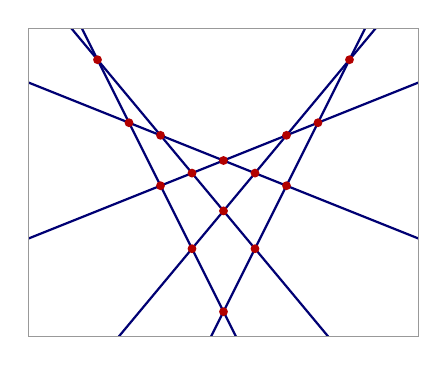
\begin{tikzpicture}[scale=0.8]
  \begin{scope}
  \clip (-3.1,-2.9) rectangle (3.1,2.0);
  \foreach \t in {-2.5,-1.5,-0.5,0.5,1.5,2.5}{
    \draw[thick,blue!45!black] (-3.2,{0.4*(2*(\t)*(-3.2)-(\t)*(\t))}) -- (3.2,{0.4*(2*(\t)*(3.2)-(\t)*(\t))});
  }
  \foreach \a/\b in {-2.5/-1.5,-2.5/-0.5,-2.5/0.5,-2.5/1.5,-2.5/2.5,-1.5/-0.5,-1.5/0.5,
                     -1.5/1.5,-1.5/2.5,-0.5/0.5,-0.5/1.5,-0.5/2.5,0.5/1.5,0.5/2.5,1.5/2.5}{
    \fill[red!70!black] ({((\a)+(\b))/2},{0.4*(\a)*(\b)}) circle (2pt);
  }
  \end{scope}
  \draw[black!40] (-3.1,-2.9) rectangle (3.1,2.0);
\end{tikzpicture}
\caption{A degenerate branch sextic: six lines in general position in the plane meet in
$\binom62=15$ points (dots). The double cover of the plane branched along the six lines has an
ordinary double point over each dot; resolving the 15 points gives a smooth K3 surface.}
\label{fig:k3:sixlines}
\end{figure}

The branch curve may degenerate. If $C$ is the union of six lines in general position
(\cref{fig:k3:sixlines}), the double cover acquires $\binom62=15$ rational double points, one
over each intersection point, and blowing them up produces a smooth K3 surface; the canonical
bundle does not change under this resolution \source{Huy ch.~1, Example~1.3(iv), ll.~267--270}.
The Euler characteristic is again $24$ (\cref{exc:k3:sixlines}).

\subsection{Kummer surfaces}\index{Kummer surface}

Let $A=\C^2/\Gamma$ be a complex two-torus and $\iota:x\mapsto-x$. The fixed points of $\iota$
are the $2^4=16$ points of order two. The quotient $A/\iota$ has 16 singular points, each
locally $\C^2/\{\pm1\}$, and its minimal resolution $X$ is a K3 surface, the Kummer surface of
$A$. \TL{} \source{Huy ch.~1, Example~1.3(iii), ll.~218--259, and Example~3.3, ll.~499--507}
The two conditions are inherited from the torus: $\dd z_1\wedge\dd z_2$ is invariant under
$\iota$ and descends to a nowhere-vanishing two-form, while $\iota$ acts as $-1$ on
$H^1(A,\mathcal{O}_A)$ (spanned by the classes of $\dd\bar z_1,\dd\bar z_2$), so nothing
invariant survives: $H^1(X,\mathcal{O}_X)=0$ although $H^1(A,\mathcal{O}_A)\neq0$.
Topologically, by the same cut-and-paste as above,
\begin{equation}\label{eq:k3:kummerchi}
  \chi(X)=\frac{\chi(A)-16}{2}+16\cdot\chi(S^2)=\frac{0-16}{2}+32=24 .
\end{equation}
This is the example closest to string theory, since $A/\iota$ is the orbifold $T^4/\Z_2$ on
which strings can be quantized exactly; \cref{ch:kummer} is devoted to it. It is also the only
one of our constructions that produces non-projective K3 surfaces, namely whenever the torus $A$
is not projective \source{Huy ch.~1, Example~3.3, ll.~508--513}.

\subsection{Elliptic K3 surfaces}\index{elliptic K3 surface}

Many K3 surfaces admit a map $\pi:X\to\mathbb{P}^1$ whose generic fibre is an elliptic curve
$y^2=4x^3-g_2x-g_3$, where $g_2$ and $g_3$ are homogeneous polynomials of degree $8$ and $12$ on
the base \source{Huy ch.~1 §4.4, ll.~721--728}. The fibre degenerates where the discriminant
$\Delta=g_2^3-27g_3^2$, of degree $24$, vanishes: generically there are $24$ singular fibres,
each a sphere with two points identified ($\chi=1$), while smooth fibres have $\chi(T^2)=0$.
Hence $\chi(X)=24$ once more. (The fibre count is standard; only the degrees of $g_2,g_3$ are
taken from the source.) In F-theory the 24 points are the positions of 24 seven-branes; the
same number controls the tadpole condition of \cref{ch:tadpole}.

\section{Hodge numbers from Riemann--Roch}\label{sec:k3:hodge}

We now forget the examples and derive the invariants from \cref{def:k3:k3} alone. The
\emph{Hodge numbers}\index{Hodge numbers} of a compact complex manifold are
\begin{equation}
  h^{p,q}(X)=\dim H^q(X,\Omega_X^p),
\end{equation}
the dimension of the space of $\bar\partial$-closed $(p,q)$-forms modulo $\bar\partial$-exact
ones. \source{Huy ch.~1 §2.4, ll.~406--410; Asp §2.1, eq.~(1), ll.~217--222} For a surface
$0\le p,q\le2$, so there are nine of them. Two general tools constrain them.

\paragraph{Serre duality.}\index{Serre duality} On a compact complex surface,
$H^q(X,E)\cong H^{2-q}(X,E^*\otimes\omega_X)^*$ for every holomorphic vector bundle $E$. With
$\omega_X\cong\mathcal{O}_X$ and $(\Omega^p_X)^*\cong\Omega_X^{2-p}$ this becomes
$h^{p,q}=h^{2-p,2-q}$: the Hodge diamond is symmetric under the rotation by $180^\circ$.

\paragraph{Hirzebruch--Riemann--Roch.}\index{Riemann--Roch theorem} For a holomorphic vector
bundle $E$ of rank $r$ on a compact complex surface, the holomorphic Euler characteristic
$\chi(X,E)=\sum_q(-1)^q\dim H^q(X,E)$ is the integral of a characteristic class,
\begin{equation}\label{eq:k3:hrr}
\begin{gathered}
  \chi(X,E)=\int_X \operatorname{ch}(E)\,\operatorname{td}(X),\\
  \operatorname{ch}(E)=r+c_1(E)+\tfrac12\big(c_1(E)^2-2c_2(E)\big),\qquad
  \operatorname{td}(X)=1+\tfrac12c_1+\tfrac1{12}\big(c_1^2+c_2\big),
\end{gathered}
\end{equation}
where $c_i=c_i(T_X)$. The left side is analytic (it counts solutions of differential
equations); the right side is topological. \source{Huy ch.~1 §2.4, eq.~(2.6), ll.~416--419; the
expansions of ch and td to degree two are standard}

\subsection{Step 1: \texorpdfstring{$\chi(\mathcal{O}_X)=2$ and Noether's formula give
$c_2=24$}{chi(O)=2 and Noether's formula give c2=24}}

By definition $h^{0,0}=1$ (holomorphic functions are constant) and $h^{0,1}=0$. Serre duality
gives $h^{0,2}=\dim H^2(X,\mathcal{O}_X)=\dim H^0(X,\omega_X)=h^{2,0}=1$. Hence
\begin{equation}\label{eq:k3:chiO}
  \chi(X,\mathcal{O}_X)=h^{0,0}-h^{0,1}+h^{0,2}=1-0+1=2 .
\end{equation}
\source{Huy ch.~1 §2.3, ll.~348--351} Now apply \eqref{eq:k3:hrr} to $E=\mathcal{O}_X$, for
which $\operatorname{ch}=1$. Only the degree-four part of the Todd class contributes to the
integral, and we obtain \emph{Noether's formula}\index{Noether's formula}
\begin{equation}\label{eq:k3:noether}
  \chi(X,\mathcal{O}_X)=\frac{c_1^2(X)+c_2(X)}{12}.
\end{equation}
For a K3 surface $c_1=0$, so $2=c_2(X)/12$, that is,
\begin{equation}\label{eq:k3:c2}
  \chi_{\mathrm{top}}(X)=\int_Xc_2(X)=24 .
\end{equation}
\source{Huy ch.~1 §2.4, ll.~420--426} This agrees with the direct count \eqref{eq:k3:chi24} on
the quartic, and with the cut-and-paste counts of \cref{sec:k3:examples}. Note what was used:
only $c_1=0$, $h^{0,1}=0$ and the uniqueness of $\Omega$.

\subsection{Step 2: no holomorphic one-forms}

For a complex K3 surface the exponential sequence $0\to\Z\to\mathcal{O}_X\to\mathcal{O}_X^*\to0$
(the second map is $f\mapsto\ee^{2\pi\ii f}$) gives a long exact sequence that begins
\begin{equation}\label{eq:k3:expseq}
  0\to H^1(X,\Z)\to H^1(X,\mathcal{O}_X)\to H^1(X,\mathcal{O}_X^*)\to H^2(X,\Z)
  \to H^2(X,\mathcal{O}_X)\to\cdots
\end{equation}
The injectivity on the left holds because $H^0(X,\mathcal{O}_X)=\C\to H^0(X,\mathcal{O}^*_X)
=\C^*$ is surjective. Since $H^1(X,\mathcal{O}_X)=0$ we get $H^1(X,\Z)=0$, hence $b_1=0$ and, by
Poincaré duality, $b_3=0$. On a compact complex surface $H^1(X,\C)\cong H^1(X,\mathcal{O}_X)
\oplus H^0(X,\Omega_X)$, so $b_1=0$ forces
\begin{equation}
  h^{1,0}=\dim H^0(X,\Omega_X)=0 ,
\end{equation}
and by Serre duality $h^{1,2}=h^{1,0}=0$, $h^{2,1}=h^{0,1}=0$. \source{Huy ch.~1 §3.2,
ll.~519--528, and §3.3, ll.~561--566} Because $T_X\cong\Omega_X$, the same statement reads
$H^0(X,T_X)=0$: a K3 surface has no holomorphic vector fields, hence no continuous group of
holomorphic symmetries.

\subsection{Step 3: \texorpdfstring{$h^{1,1}=20$}{h11 = 20}}

Apply \eqref{eq:k3:hrr} to $E=\Omega_X$, of rank two. Its Chern classes are
$c_1(\Omega_X)=-c_1(T_X)=0$ and $c_2(\Omega_X)=c_2(T_X)$, with $\int c_2=24$. Therefore
$\operatorname{ch}(\Omega_X)=2-c_2$ and
\begin{equation}\label{eq:k3:chiOmega}
  \chi(X,\Omega_X)=\int_X\big(2-c_2\big)\Big(1+\frac{c_2}{12}\Big)
  =2\cdot\frac{24}{12}-24=-20 .
\end{equation}
On the other hand $\chi(X,\Omega_X)=h^{1,0}-h^{1,1}+h^{1,2}=-h^{1,1}$ by Step~2. Hence
\begin{equation}\label{eq:k3:h11}
  h^{1,1}(X)=20 .
\end{equation}
\source{Huy ch.~1 §2.4, ll.~427--432 (there written as $2h^0(\Omega_X)-h^1(\Omega_X)=-20$)}

\begin{figure}[t]
\centering
\begin{tikzpicture}[x=1.15cm,y=0.95cm]
  \node (h00) at (0,2) {$1$};
  \node (h10) at (-1,1) {$0$}; \node (h01) at (1,1) {$0$};
  \node (h20) at (-2,0) {$1$}; \node (h11) at (0,0) {$\mathbf{20}$}; \node (h02) at (2,0) {$1$};
  \node (h21) at (-1,-1) {$0$}; \node (h12) at (1,-1) {$0$};
  \node (h22) at (0,-2) {$1$};
  \node[font=\scriptsize,black!60] at (0,2.45) {$h^{0,0}$};
  \node[font=\scriptsize,black!60] at (-2.55,0) {$h^{2,0}$};
  \node[font=\scriptsize,black!60] at (2.55,0) {$h^{0,2}$};
  \node[font=\scriptsize,black!60] at (0,-2.45) {$h^{2,2}$};
  \node[font=\scriptsize,black!60] at (0,-0.45) {$h^{1,1}$};
  \draw[dashed,black!45] (0,1.6)--(0,0.4); \draw[dashed,black!45] (0,-0.8)--(0,-1.6);
  \draw[<->,blue!50!black] (-0.75,1) -- node[above,font=\scriptsize,pos=0.5,fill=white,
      inner sep=1pt,yshift=2pt] {$p\leftrightarrow q$} (0.75,1);
  % Betti numbers
  \foreach \y/\b/\v in {2/0/1,1/1/0,0/2/22,-1/3/0,-2/4/1}{
    \node[font=\small] at (4.3,\y) {$b_{\b}=\v$};
    \draw[black!25] (2.9,\y)--(3.6,\y);
  }
  \node[font=\small] at (4.3,-2.8) {$\chi=24$};
\end{tikzpicture}
\caption{The Hodge diamond of a K3 surface. Row $k$ (from the top, $k=0,\dots,4$) lists
$h^{p,q}$ with $p+q=k$ and sums to the Betti number $b_k$. Reflection in the dashed vertical
axis is complex conjugation, $h^{p,q}=h^{q,p}$; rotation by $180^\circ$ is Serre duality,
$h^{p,q}=h^{2-p,2-q}$.}
\label{fig:k3:diamond}
\end{figure}

\subsection{The Hodge diamond and the Betti numbers}

The nine numbers are customarily arranged in a diamond\index{Hodge diamond}, with $h^{p,q}$
in row $p+q$; see \cref{fig:k3:diamond}.
\source{Huy ch.~1, eq.~(2.7), ll.~437--447; Asp §2.1, eq.~(14), ll.~377--404} The diamond is
the same for every K3 surface, projective or not, and over any field. Since a K3 surface is
Kähler, the Hodge decomposition $H^k(X,\C)=\bigoplus_{p+q=k}H^{p,q}(X)$ holds and the rows of
the diamond sum to the Betti numbers (\cref{fig:k3:diamond}):
\begin{equation}\label{eq:k3:betti}
  b_0=1,\quad b_1=0,\quad b_2=h^{2,0}+h^{1,1}+h^{0,2}=22,\quad b_3=0,\quad b_4=1 .
\end{equation}
There are two checks. First, $\sum_k(-1)^kb_k=1+22+1=24$ reproduces \eqref{eq:k3:c2}; read
the other way, $\chi=24$ and $b_1=b_3=0$ give $b_2=22$ without Hodge theory
\source{Huy ch.~1 §3.3, ll.~576--585}. Second, for the quartic the row $n=4$ of the table in
\cref{ex:k3:degrees} gave the same $b_2=22$ from a Chern class computation on $\mathbb{P}^3$.
(This is Aspinwall's route to $h^{1,1}=22-2=20$ \source{Asp §2.1, ll.~370--379}.)

Moreover $H^2(X,\Z)$ has no torsion, so
\begin{equation}
  H^2(X,\Z)\cong\Z^{22}.
\end{equation}
\source{Huy ch.~1 §3.2, ll.~535--540, and §3.3, l.~586} \TL{}

\begin{physicsbox}[What the Hodge numbers count in physics]
When a ten-dimensional field theory is compactified on $X$, massless fields in the
lower-dimensional theory come from harmonic forms on $X$, and there are $b_k$ independent
harmonic $k$-forms. For K3, $b_1=0$ means that the metric or a vector potential with one leg
along $X$ yields no massless vectors, in line with the absence of continuous isometries;
$b_2=22$ means that a two-form field such as $B$ gives $22$ massless scalars, one for each
two-cycle. The split $22=1+20+1$ also has a meaning: deformations of the complex structure are
counted by $H^1(X,T_X)\cong H^1(X,\Omega_X)$, of dimension $h^{1,1}=20$, again because
$T_X\cong\Omega_X$. The resulting moduli space is the subject of \cref{ch:stringsk3}.
\end{physicsbox}

\subsection{Line bundles and curves: a first look at the Picard lattice}

For a line bundle $L$ formula \eqref{eq:k3:hrr} with $c_1(X)=0$ reads
\begin{equation}\label{eq:k3:rrline}
  \chi(X,L)=\frac{(L)^2}{2}+2,
\end{equation}
where $(L)^2=\int_Xc_1(L)^2$ is the self-intersection number \source{Huy ch.~1 §2.3,
eq.~(2.5), ll.~359--361}. Since the left side is an integer, $(L)^2$ is even for every line
bundle. If $C\subset X$ is a smooth curve of genus $g$, the adjunction formula
$2g-2=(C)^2+K\cdot C$ with $K=0$ gives
\begin{equation}
  (C)^2=2g-2 :
\end{equation}
a rational curve ($g=0$) on a K3 surface has self-intersection $-2$\index{(-2)-curve}, as have
the 16 exceptional spheres of a Kummer surface. The exact sequence \eqref{eq:k3:expseq} also
identifies the group of line bundles $\operatorname{Pic}(X)=H^1(X,\mathcal{O}_X^*)$ with the
kernel of $H^2(X,\Z)\to H^2(X,\mathcal{O}_X)$, the integral classes of type $(1,1)$:
\begin{equation}\label{eq:k3:picard}
  \operatorname{Pic}(X)\cong H^2(X,\Z)\cap H^{1,1}(X),\qquad
  \rho(X):=\rk\operatorname{Pic}(X)\le h^{1,1}=20 .
\end{equation}
\source{Huy ch.~1 §3.3, eqs.~(3.2)--(3.3), ll.~568--575} The \emph{Picard
number}\index{Picard number} $\rho$ depends on the complex structure and takes every value
from $0$ to $20$. \TL{} It returns in \cref{ch:k3lattice}.

\section{The intersection form: unimodular, even, signature \texorpdfstring{$(3,19)$}{(3,19)}}
\label{sec:k3:signature}

On a compact oriented four-manifold the cup product defines a symmetric bilinear form on
$H^2(X,\Z)$ modulo torsion,
\begin{equation}
  (\alpha,\beta)=\int_X\alpha\wedge\beta\in\Z ,
\end{equation}
equal to the number of intersection points, counted with orientation, of two surfaces
representing the dual homology classes \source{Asp §2.3, eq.~(19), ll.~514--522}. For a K3
surface this makes $\Z^{22}$ into a lattice in the sense of \cref{ch:lattices}, the
\emph{K3 lattice}\index{K3 lattice}. It has three properties, which together determine it.

\subsection{Unimodular}

Poincaré duality states that for a basis $\{e_i\}$ of $H_2(X,\Z)$ there is a dual basis
$\{e_j^*\}$ of $H_2(X,\Z)$ with $(e_i,e^*_j)=\delta_{ij}$. Hence the Gram matrix of the
intersection form is invertible over $\Z$ and has determinant $\pm1$: the lattice is
unimodular (self-dual)\index{unimodular lattice}. \source{Asp §2.3, ll.~537--542; Huy ch.~1
§3.3, ll.~586--588}

\subsection{Signature by the Hirzebruch signature theorem}
\index{Hirzebruch signature theorem}\index{signature!of K3}

Let $b_+$ and $b_-$ be the numbers of positive and negative eigenvalues of the form on
$H^2(X,\R)$, and $\sigma=b_+-b_-$ its signature (the \emph{index}). The signature theorem
expresses $\sigma$ by the first Pontryagin class, $\sigma=\frac13\int_Xp_1$, and for a complex
surface $p_1=c_1^2-2c_2$. Therefore
\begin{equation}\label{eq:k3:hirzebruch}
  \sigma(X)=\frac{c_1^2-2c_2}{3}=\frac{0-2\cdot24}{3}=-16 .
\end{equation}
\source{Huy ch.~1, proof of Prop.~3.5, ll.~614--619; Asp §2.3, eq.~(20), ll.~523--536, in the
form $\sigma=-\frac23\chi$} Together with $b_++b_-=22$,
\begin{equation}\label{eq:k3:319}
  b_+=\frac{22-16}{2}=3,\qquad b_-=\frac{22+16}{2}=19 .
\end{equation}

\subsection{Signature again, from Hodge theory}

The number $b_+=3$ can be understood form by form. Let $J$ be a Kähler form on $X$ and
$\Omega$ the holomorphic two-form. Work at a point in flat coordinates $z_1=x_1+\ii x_2$,
$z_2=x_3+\ii x_4$, with $e_i=\dd x_i$ and volume form $\mathrm{vol}=e_1\wedge e_2\wedge
e_3\wedge e_4$, in which $J=\frac{\ii}{2}(\dd z_1\wedge\dd\bar z_1+\dd z_2\wedge\dd\bar z_2)$
and $\Omega=\dd z_1\wedge\dd z_2$. Expanding,
\begin{equation}\label{eq:k3:sdforms}
\begin{aligned}
  J&=e_1\wedge e_2+e_3\wedge e_4,\\
  \operatorname{Re}\Omega&=e_1\wedge e_3-e_2\wedge e_4=e_1\wedge e_3+e_4\wedge e_2,\\
  \operatorname{Im}\Omega&=e_1\wedge e_4+e_2\wedge e_3 .
\end{aligned}
\end{equation}
These are exactly the three self-dual two-forms of $\R^4$ (those with $*\alpha=\alpha$)
\source{Asp §2.4, eq.~(37), ll.~824--837}. Each squares to $\alpha\wedge\alpha=2\,
\mathrm{vol}>0$, and they are mutually orthogonal, e.g.\ $J\wedge\operatorname{Re}\Omega=0$
because no term of the product contains all four $e_i$. Globally,
\begin{equation}
  \int_XJ\wedge J=2\operatorname{Vol}(X)>0,\qquad
  \int_X\Omega\wedge\bar\Omega>0,\qquad \int_X\Omega\wedge\Omega=0,\qquad
  \int_XJ\wedge\Omega=0,
\end{equation}
the last two for reasons of type: a $(4,0)$- or $(3,1)$-form on a surface vanishes. So the
classes $[J]$, $[\operatorname{Re}\Omega]$, $[\operatorname{Im}\Omega]$ span a positive
definite three-plane in $H^2(X,\R)$ \source{Asp §2.4, ll.~835--857}. The Hodge index
theorem\index{Hodge index theorem} says that there is nothing more: on the orthogonal
complement of $[J]$ inside $H^{1,1}$ the form is negative definite (in the flat model, the
$(1,1)$-form $e_1\wedge e_2-e_3\wedge e_4$ is orthogonal to $J$, anti-self-dual, and squares to
$-2\,\mathrm{vol}$). For any compact Kähler surface this gives
\begin{equation}\label{eq:k3:hodgeindex}
  b_+=2h^{2,0}+1,\qquad b_-=h^{1,1}-1,
\end{equation}
which for K3 is $(b_+,b_-)=(3,19)$ and $\sigma=2+2-20=-16$, in agreement with
\eqref{eq:k3:hirzebruch}. (Formula \eqref{eq:k3:hodgeindex} is standard; our sources state the index theorem for
$H^{1,1}$ \source{Huy ch.~1, Remark~3.4, ll.~547--558} and the dimensions $3$ and $19$
\source{Asp §2.4, eqs.~(35)--(36), ll.~807--816}.) The row
$n=5$ of \cref{ex:k3:degrees} offers an independent test of \eqref{eq:k3:hodgeindex}: there
$h^{2,0}=\chi(\mathcal{O})-1=4$ and indeed $b_+=9=2\cdot4+1$.

\subsection{Even}

Finally, $(\alpha,\alpha)\in2\Z$ for all $\alpha\in H^2(X,\Z)$: the lattice is
even\index{even lattice}. For classes of line bundles we saw this in \eqref{eq:k3:rrline},
but line bundles span at most a sublattice of rank $20$. The general statement is topological:
by Wu's formula the intersection form of a closed oriented smooth four-manifold is even if
and only if the second Stiefel--Whitney class $w_2$ vanishes, and for a complex surface
$w_2\equiv c_1\pmod 2$. A K3 surface has $c_1=0$, so its form is even. \TL{}
\source{Huy ch.~1, proof of Prop.~3.5, ll.~610--613; Asp §2.3, ll.~543--551} The condition
$w_2=0$ is also the condition for spinors to exist on $X$, which we need in
\cref{sec:k3:holonomy}. The quartic is the only even row in the table of
\cref{ex:k3:degrees} besides the quadric: $c_1=(4-n)x$ is even exactly for even $n$.

\subsection{The result}

Indefinite even unimodular lattices are classified by their signature (\cref{ch:lattices}):
$b_+-b_-$ must be divisible by $8$ and the lattice is then unique. For $(3,19)$ this gives:

\begin{theorem}[The K3 lattice]\label{thm:k3:lattice}
For a complex K3 surface $X$, the group $H^2(X,\Z)$ with its intersection form is an even
unimodular lattice of signature $(3,19)$, and hence
\begin{equation}\label{eq:k3:lattice}
  H^2(X,\Z)\;\cong\;U\oplus U\oplus U\oplus E_8(-1)\oplus E_8(-1).
\end{equation}
\TL{} \source{Huy ch.~1, Prop.~3.5, ll.~600--619}
\end{theorem}

The bookkeeping is: rank $3\cdot2+2\cdot8=22$; each hyperbolic plane $U$ has signature
$(1,1)$ and each $E_8(-1)$ has signature $(0,8)$, giving $(3,\,3+16)=(3,19)$ and
$\sigma=-16=2\cdot(-8)$. The isomorphism \eqref{eq:k3:lattice} is abstract; exhibiting 22
explicit cycles with this Gram matrix is best done on a Kummer surface (\cref{ch:kummer}).

\begin{pitfallbox}[Signs and orientations]
Which of $3$ and $19$ counts the positive directions depends on the orientation. We use the
orientation given by the complex structure, for which $\int J\wedge J>0$; with it the
self-dual harmonic forms are the three positive directions and $E_8$ enters with its
\emph{negative} definite form, written $E_8(-1)$ or $-E_8$. Reversing the orientation turns
$(3,19)$ into $(19,3)$ and $\sigma$ into $+16$. Also do not confuse $\chi_{\mathrm{top}}=24$ with $\chi(\mathcal{O}_X)=2$; Noether's
formula \eqref{eq:k3:noether} relates them, $24=12\cdot2$.
\end{pitfallbox}

\section{Holonomy, hyperkähler structure and supersymmetry}\label{sec:k3:holonomy}

\subsection{Ricci-flat metrics and \texorpdfstring{$SU(2)$}{SU(2)} holonomy}

So far no metric was used. Physics needs one: a string background must, to lowest order in
$\ap$, solve the vacuum Einstein equations $R_{\mu\nu}=0$ (\cref{ch:backgrounds}). For a
Kähler metric the Ricci tensor defines a closed $(1,1)$-form representing $2\pi c_1(T_X)$
(a standard fact), so $c_1=0$ is necessary for Ricci-flatness. Yau's theorem\index{Yau's theorem} states that it is
sufficient: on a compact Kähler manifold with $K=0$ and a fixed complex structure, every Kähler
class contains a unique Ricci-flat Kähler metric. \TL{} \source{Asp §2.4, ll.~841--843} No such
metric on a K3 surface is known in closed form \source{Asp §2.4, ll.~860--862}; what follows
uses only its existence.

The \emph{holonomy group}\index{holonomy} of a Riemannian manifold $M$ of dimension $d$ is the
group of all linear maps of a tangent space $T_pM$ obtained by parallel transport, with the
Levi-Civita connection, around closed loops based at $p$. It is a subgroup of $O(d)$, of
$SO(d)$ if $M$ is orientable, and special geometries correspond to smaller subgroups: the
holonomy lies in $U(d/2)$ if and only if the metric is Kähler, in $SU(d/2)$ if and only if it is
Ricci-flat Kähler (Calabi--Yau), and in $Sp(d/4)$ if and only if it is hyperkähler
\source{Asp §2.2, ll.~410--434}. The logic is that a tensor is covariantly constant if and only
if it is invariant under the holonomy group: $U(d/2)$ is the subgroup of $SO(d)$ preserving a
complex structure, $SU(d/2)$ preserves in addition a holomorphic volume form, and $Sp(d/4)$
preserves a quaternionic structure. For $d=4$ the last two coincide, $SU(2)\cong Sp(1)$, so:

\begin{proposition}\label{prop:k3:hyperkahler}
A K3 surface with its Ricci-flat Kähler metric has holonomy $SU(2)$ and is
hyperkähler\index{hyperkähler manifold}: the metric is Kähler with respect to a whole
two-sphere of complex structures $aI+bJ+cK$, $a^2+b^2+c^2=1$, where $I,J,K$ satisfy the
quaternion relations. \TL{} \source{Asp §2.2, ll.~472--482; §2.4, ll.~870--874}
\end{proposition}

The sphere is visible in \eqref{eq:k3:sdforms}. The rotation group of $\R^4$ is locally a
product, $SO(4)\cong(SU(2)_+\times SU(2)_-)/\Z_2$. A vector transforms as $(\mathbf2,\mathbf2)$
and the six-dimensional space of two-forms splits as
\begin{equation}\label{eq:k3:twoforms}
  \Lambda^2\R^4=\Lambda^+\oplus\Lambda^-=(\mathbf3,\mathbf1)\oplus(\mathbf1,\mathbf3),
\end{equation}
self-dual plus anti-self-dual. If the holonomy group is $SU(2)_-$, it acts trivially on
$\Lambda^+$: the bundle of self-dual two-forms is flat, and because $X$ is simply connected it
has three globally defined covariantly constant sections, $J$, $\operatorname{Re}\Omega$ and
$\operatorname{Im}\Omega$ \source{Asp §2.4, ll.~819--823}. Covariantly constant forms are
harmonic, and we recover $b_+=3$: \emph{the three positive directions of the K3 lattice are
the three parallel two-forms of the hyperkähler metric}. An $SO(3)$ rotation of the triple
does not change the metric but changes which combination is called the Kähler form and which
the holomorphic two-form; these rotations sweep out the two-sphere of complex structures.
The dimension count $\dim SU(2)=3<6=\dim SO(4)$, with a complement of dimension $3$, is the
only part of this paragraph that has a counterpart in Lean (\cref{sec:k3:lean}).

\subsection{Why K3 preserves half of the supersymmetry}\index{supersymmetry!on K3}

A supersymmetry of the compactified theory requires a covariantly constant spinor on $X$:
the supersymmetry parameter must be invariant under parallel transport, that is, under the
holonomy group. A Dirac spinor in four Euclidean dimensions has four components, two of each
chirality, transforming as
\begin{equation}\label{eq:k3:spinor4}
  \mathbf4=(\mathbf2,\mathbf1)\oplus(\mathbf1,\mathbf2)
  \quad\text{under}\quad SU(2)_+\times SU(2)_- .
\end{equation}
On a generic four-manifold the holonomy is all of $SO(4)$, neither summand contains an
invariant, and no supersymmetry survives. On a flat torus the holonomy is trivial and all four
components are constant. On K3 the holonomy $SU(2)_-$ leaves the two components of
$(\mathbf2,\mathbf1)$ invariant and mixes the other two. In ten dimensions, the
$16$-component Majorana--Weyl supercharge decomposes under $so(1,9)\supset so(1,5)\oplus
su(2)_+\oplus su(2)_-$ as
\begin{equation}\label{eq:k3:16}
  \mathbf{16}\;\to\;(\mathbf4,\mathbf2,\mathbf1)\oplus(\mathbf4',\mathbf1,\mathbf2),
\end{equation}
and only the first summand, with $4\cdot2=8$ of the $16$ components, is invariant under the
holonomy. \source{Asp §4.1, eq.~(89), ll.~2273--2295} The rule is:
\begin{quote}
\emph{Compactification on a smooth K3 surface preserves half as many supersymmetries as
compactification on a torus $T^4$.}
\end{quote}
The heterotic and type~I strings, with $16$ supercharges in ten dimensions, keep $8$ on K3,
which is the minimal supersymmetry in six dimensions \source{Asp §4.1, ll.~2288--2293}; the
type~II strings, with $32$, keep $16$.

\begin{physicsbox}[Why physicists love K3]
Half of the supersymmetry is the useful amount. With all of it (tori) everything is fixed by
symmetry; with a quarter or less (Calabi--Yau threefolds) quantum corrections are hard to
control. With half, the moduli space of the compactified theory is still determined exactly by
symmetry and by the lattice $H^2(X,\Z)$, yet the internal space is curved, has no isometries
and has a rich topology. K3 is therefore the simplest laboratory for exact statements about
strings on curved spaces, such as string dualities (\cref{ch:stringsk3}). It is also the only
one of its kind: a compact Ricci-flat Kähler surface whose holonomy is exactly $SU(2)$ is a K3
surface (standard; not checked against a source in this book's library).
\end{physicsbox}

\begin{remark}[The Dirac index]\label{rem:k3:dirac}
The two parallel spinors can be counted topologically. On a spin four-manifold the index of
the Dirac operator is $-\frac1{24}\int p_1=-\sigma/8$, which for K3 equals $16/8=2$. For a
Kähler surface with $c_1=0$ this is the Todd genus $\chi(\mathcal{O}_X)=c_2/12=2$ of
\eqref{eq:k3:chiO}: positive-chirality spinors are sections of
$\Lambda^{0,0}\oplus\Lambda^{0,2}$, with zero modes $1$ and $\bar\Omega$. (Standard index
theory; not checked against a source in this book's library. The arithmetic $16/8=2$ appears in
Lean, \cref{sec:k3:lean}.)
\end{remark}

\section{What the machine has checked}\label{sec:k3:lean}

It is important to be precise here, because the distance between the mathematics of this
chapter and its formal counterpart is larger than anywhere in Parts~II and~III. \emph{No
complex manifold, sheaf, cohomology group, Chern class or metric is defined in any of the Lean
libraries of this project.} A faithful formalization of $\chi(K3)=24$ would need compact complex
surfaces, coherent sheaf cohomology with Serre duality, Chern classes and the
Hirzebruch--Riemann--Roch theorem, which the project does not supply. The four files attached
to this chapter contain the \emph{arithmetic shadow} of
\cref{sec:k3:hodge,sec:k3:signature,sec:k3:holonomy}: the numbers $1,0,20,22,24,3,19,-16$ are
entered as data, and the kernel checks that they are consistent with each other under the
formulas of this chapter. Every statement above about actual K3 surfaces is therefore Tier~L.
All declarations below depend on no axioms beyond \lean{propext}, \lean{Classical.choice} and
\lean{Quot.sound}.

\subsection{The Hodge table and its checksums}

The file \texttt{Frontier/HodgeNumbers.lean} of the library
\texttt{StringTheoryFormalization} (namespace \lean{StringTheory.Frontier}) stores the diamond of \cref{fig:k3:diamond} as a function on
$\{0,1,2\}^2$:

\begin{leancode}
def k3HodgeNumber : Fin 3 → Fin 3 → ℕ
  | ⟨0, _⟩, ⟨0, _⟩ => 1   -- h^{0,0} = 1
  | ⟨0, _⟩, ⟨1, _⟩ => 0   -- h^{0,1} = 0
  | ⟨0, _⟩, ⟨2, _⟩ => 1   -- h^{0,2} = 1
  | ⟨1, _⟩, ⟨0, _⟩ => 0   -- h^{1,0} = 0
  | ⟨1, _⟩, ⟨1, _⟩ => 20  -- h^{1,1} = 20
  | ⟨1, _⟩, ⟨2, _⟩ => 0   -- h^{1,2} = 0
  | ⟨2, _⟩, ⟨0, _⟩ => 1   -- h^{2,0} = 1
  | ⟨2, _⟩, ⟨1, _⟩ => 0   -- h^{2,1} = 0
  | ⟨2, _⟩, ⟨2, _⟩ => 1   -- h^{2,2} = 1

theorem k3_euler_characteristic :
    (∑ p : Fin 3, ∑ q : Fin 3,
      (if (p.val + q.val) % 2 = 0 then 1 else -1 : ℤ) *
      (k3HodgeNumber p q : ℤ)) = 24 := by ...

theorem k3_hodge_symmetry (p q : Fin 3) :
    k3HodgeNumber p q = k3HodgeNumber q p := by ...

theorem k3_serre_duality (p q : Fin 3) :
    k3HodgeNumber p q =
      k3HodgeNumber ⟨2 - p.val, by omega⟩ ⟨2 - q.val, by omega⟩ := by ...

theorem k3_b2 :
    k3HodgeNumber ⟨0, by norm_num⟩ ⟨2, by norm_num⟩ +
    k3HodgeNumber ⟨1, by norm_num⟩ ⟨1, by norm_num⟩ +
    k3HodgeNumber ⟨2, by norm_num⟩ ⟨0, by norm_num⟩ = 22 := by ...
\end{leancode}

\begin{leanbox}[In Lean: a nine-entry table sums to 24 and to 22]
\textbf{Reading.} \lean{k3HodgeNumber} is a definition by cases, a lookup table; the number $20$
in it is typed in, not derived. \lean{k3\_euler\_characteristic} says that
$\sum_{p,q}(-1)^{p+q}h^{p,q}=24$ for this table, the Hodge-theoretic form of $\chi=\sum(-1)^kb_k$.
\lean{k3\_hodge\_symmetry} and \lean{k3\_serre\_duality} say that the table is invariant under
$(p,q)\mapsto(q,p)$ and $(p,q)\mapsto(2-p,2-q)$; \lean{k3\_b2} says that its middle row sums to
$22$. \textbf{Proof idea.} The sums are expanded with \texttt{Fin.sum\_univ\_three} and
evaluated by \texttt{simp}; the two symmetries are checked on all nine pairs by
\texttt{fin\_cases p <;> fin\_cases q <;> rfl}. \textbf{What it is not.} These are checksums on
the table: a typing error in one entry would very likely break one of them. They are not proofs
of Noether's formula, of Hodge symmetry or of Serre duality, which are theorems about all
compact Kähler manifolds and need the objects listed above. The file also contains \lean{hodge11\_from\_kummer}, which despite its name checks only
that the entry $20$ equals $|\lean{Fin 16}|+4$, that is, $20=16+4$.
\end{leanbox}

\subsection{Signature from the table}

The file \texttt{UseCases/K3SignatureTheorem.lean} of the same library (namespace\\
\lean{StringTheory.UseCases.K3Signature}) takes the Hodge-index route
\eqref{eq:k3:hodgeindex}, not the Hirzebruch route \eqref{eq:k3:hirzebruch}:

\begin{leancode}
def bPlus : ℕ := 2 * k3HodgeNumber ⟨2, by norm_num⟩ ⟨0, by norm_num⟩ + 1
def bMinus : ℕ := k3HodgeNumber ⟨1, by norm_num⟩ ⟨1, by norm_num⟩ - 1

theorem bPlus_eq_three : bPlus = 3 := by ...
theorem bMinus_eq_nineteen : bMinus = 19 := by ...
theorem betti_sum_eq_b2 : bPlus + bMinus = 22 := by ...
theorem k3_signature_eq_neg_sixteen :
    (bPlus : ℤ) - (bMinus : ℤ) = -16 := by ...
\end{leancode}

\begin{leanbox}[In Lean: $2\cdot1+1=3$, $20-1=19$, $3-19=-16$]
\textbf{Reading.} \lean{bPlus} and \lean{bMinus} are \emph{defined} by the right-hand sides of
\eqref{eq:k3:hodgeindex}, evaluated on the table. The theorems say that these natural numbers are
$3$ and $19$, that they add up to $22$, and that their difference, computed in $\Z$, is $-16$.
\textbf{Proof idea.} Unfold the definitions and let \texttt{decide} evaluate; the sum is
rewritten into the three table entries of \lean{k3\_b2} and closed by that theorem, so
$b_++b_-=b_2$ is a genuine dependency and not a second copy of the number $22$; the last step
is \texttt{norm\_num}. \textbf{What it is not.} The Hodge index theorem is the content of the
\emph{definition}, which the kernel cannot check: had we defined \lean{bPlus} as $2h^{2,0}+2$, Lean
would prove $\sigma=-14$ without complaint. Neither an intersection form nor the signature
theorem appears. The cast to $\Z$ matters: in $\N$, truncated subtraction gives $3-19=0$.
\end{leanbox}

\subsection{Two older libraries: the same numbers as bare integers}

Two files of the older libraries described in \cref{ch:architecture} define small arithmetic
functions and evaluate them at the K3 values. The first is
\texttt{DoubleFieldTheory/K3Topology.lean}, with namespace \lean{DoubleFieldTheory.K3Topology}:

\begin{leancode}
def K3BettiSum (b0 b1 b2 b3 b4 : Int) : Int :=
  b0 - b1 + b2 - b3 + b4
theorem k3_euler_characteristic :
    K3BettiSum 1 0 22 0 1 = 24 := by decide

def LatticeRank (n_e8 n_u : Int) : Int := n_e8 * 8 + n_u * 2
def LatticeSig (n_e8 n_u : Int) : Int := n_e8 * (-8) + n_u * 0
theorem k3_intersection_lattice_rank_sig :
    LatticeRank 2 3 = 22 ∧ LatticeSig 2 3 = -16 := by decide

def DiracIndex (sig : Int) : Int := (-sig) / 8
theorem k3_atiyah_singer_dirac_index :
    DiracIndex (-16) = 2 := by decide
\end{leancode}

\noindent Further evaluations of the same kind, in this file and in
\texttt{StringTheoryFoundation/K3/}\allowbreak\texttt{K3Surfaces.lean}, which stores the diamond
as a record with nine fields:
\begin{center}\small
\begin{tabular}{@{}lll@{}}
\toprule
declaration & file & content\\
\midrule
\lean{k3\_hirzebruch\_signature} & \texttt{K3Topology} & $3-19=-16$\\
\lean{k3\_su2\_holonomy\_reduction} & \texttt{K3Topology} & $3<6$ and $6-3=3$
   (constants for $su(2)$, $so(4)$)\\
\lean{k3\_lattice\_rank\_valid} & \texttt{K3Surfaces} & $3\cdot2+2\cdot8=22$\\
\lean{k3\_signature\_is\_minus\_16} & \texttt{K3Surfaces} & $3-19=-16$ in $\Z$\\
\bottomrule
\end{tabular}
\end{center}

\begin{leanbox}[In Lean: evaluations of integer formulas]
\textbf{Reading.} Each theorem evaluates an explicit integer expression:
$1-0+22-0+1=24$; $2\cdot8+3\cdot2=22$ and $2\cdot(-8)+3\cdot0=-16$, the rank and
signature bookkeeping below \cref{thm:k3:lattice}; $16/8=2$, the arithmetic of
\cref{rem:k3:dirac}. \textbf{Proof idea.}
\texttt{decide} or \texttt{rfl}: the kernel computes both sides. \textbf{What it is not.} The
names \lean{k3\_hirzebruch\_signature} and \lean{k3\_atiyah\_singer\_dirac\_index} refer to
the theorems that \emph{motivate} the formulas; the formulas themselves are definitions, and
neither theorem is stated. \lean{LatticeRank} counts summands and does not mention a lattice;
the lattices $U$ and $E_8$ with their Gram matrices live in a different library
(\cref{ch:lattices}). One detail deserves a warning: \lean{DiracIndex} uses integer division,
which rounds, so \lean{DiracIndex (-15)} also evaluates to an integer although no spin
four-manifold has signature $-15$.
A companion statement, \lean{k3\_parallel\_chiral\_spinor\_index}, checks $2-0=2$.
\end{leanbox}

\subsection{The atlas finding: one fact, several proofs}

The project's theorem atlas (\cref{ch:atlas}) compares all statements across libraries by
textual similarity and by shared dependencies. The fact $\chi(K3)=24$ is its clearest example
of duplication. It is proved independently five times:
\begin{center}\small
\begin{tabular}{@{}ll@{}}
\toprule
declaration & starting point\\
\midrule
\lean{DoubleFieldTheory.K3Topology.k3\_euler\_characteristic} & Betti numbers as arguments\\
\lean{StringTheory.Frontier.k3\_euler\_characteristic} & the Hodge table\\
\lean{SocrateAI.Moonshine.k3\_euler\_eq\_24} & constants \lean{k3\_b0}, \dots, \lean{k3\_b4}\\
\lean{Lean5Corpus.Problems.KummerModularity.}\\
\quad\lean{k3\_euler\_characteristic\_identity} & $1+22+1$ equals a constant set to $24$\\
\lean{StringTheory.Foundation.Atlas.}\\
\quad\lean{atlas\_k3\_euler\_characteristic} & fields of a record \lean{defaultK3}\\
\bottomrule
\end{tabular}
\end{center} The first and third have
the highest cross-library statement similarity in the whole atlas (cosine $0.631$), while the
first two share almost no dependencies (dependency overlap $0.009$). \source{atlas.md, section
``Most similar statements across libraries''} Agreement between such proofs is weak evidence: each starts from its own hand-entered copy of
the Betti or Hodge numbers, so the five proofs confirm five times that $1+22+1=24$, not that
$b_2(K3)=22$.

The newer library does it differently. \lean{k3HodgeNumber} is one of the atlas hubs, used by
twelve theorems, and the statements that need K3 data import that single table instead of
retyping it:

\begin{leancode}
-- DualScaleStream2/Flux/Tadpole.lean
theorem euler_K3 :
    eulerFromHodge StringTheory.Frontier.k3HodgeNumber = 24 := by ...

-- DualScaleStream2/Lattice/K3T2Signature.lean
theorem sigK3_matches_hodge :
    sigK3.pos = StringTheory.UseCases.K3Signature.bPlus ∧
    sigK3.neg = StringTheory.UseCases.K3Signature.bMinus := by ...
\end{leancode}

\noindent The second statement is the more interesting one. Its left side is the signature
$(3,19)$ computed from the decomposition $3U\oplus2E_8(-1)$, its right side is
\eqref{eq:k3:hodgeindex} evaluated on the Hodge table. It is a machine-checked consistency
check between two independently tabulated literature inputs, the formal counterpart of our
remark that \eqref{eq:k3:hirzebruch} and \eqref{eq:k3:hodgeindex} agree.

\subsection{Tier table}

\begin{center}
\small
\begin{tabular}{@{}p{0.47\textwidth}cp{0.41\textwidth}@{}}
\toprule
Statement & Tier & Evidence\\
\midrule
The examples of \cref{sec:k3:examples} are K3; all K3 are diffeomorphic & \TL & Huy ch.~1,
Ex.~1.3, Rem.~3.6; Asp Thm.~1\\
$\chi=24$, Hodge diamond, $b_2=22$; $H^2(X,\Z)\cong3U\oplus2E_8(-1)$ & \TL & Huy ch.~1
§2.4, §3.3, Prop.~3.5; Asp §2.1\\
Ricci-flat metric, holonomy $SU(2)$, half of the supersymmetry & \TL & Asp §2.2, §2.4, §4.1\\
\addlinespace
The table \lean{k3HodgeNumber} has alternating sum $24$, middle row $22$, and both
symmetries & \TA & \lean{k3\_euler\_characteristic}, \lean{k3\_b2},
\lean{k3\_hodge\_symmetry}, \lean{k3\_serre\_duality}\\
$2h^{2,0}+1=3$, $h^{1,1}-1=19$, difference $-16$, on that table & \TA &
\lean{bPlus\_eq\_three}, \lean{bMinus\_eq\_nineteen}, \lean{k3\_signature\_eq\_neg\_sixteen}\\
Lattice-side and Hodge-side $(b_+,b_-)$ agree & \TA & \lean{sigK3\_matches\_hodge}\\
$1-0+22-0+1=24$, $3-19=-16$, $2\cdot8+3\cdot2=22$, $16/8=2$ & \TA &
\lean{DoubleFieldTheory.K3Topology}, \lean{K3Surfaces}\\
\addlinespace
The table \emph{is} the Hodge diamond of a K3 surface & --- & identification; by the rules of
this book never Tier~A\\
\bottomrule
\end{tabular}
\end{center}

\begin{summarybox}
\begin{itemize}[leftmargin=*,itemsep=1pt]
\item A K3 surface is a compact complex surface with trivial canonical bundle and
  $H^1(X,\mathcal{O}_X)=0$. It carries a nowhere-vanishing holomorphic two-form $\Omega$,
  unique up to scale, and $T_X\cong\Omega_X$. Examples: quartics in $\mathbb{P}^3$, complete
  intersections $(2,3)$ and $(2,2,2)$, double planes branched over a sextic, Kummer surfaces,
  elliptic fibrations with 24 singular fibres. All are diffeomorphic.
\item $\chi(\mathcal{O}_X)=2$ and Noether's formula give $\chi=c_2=24$; Riemann--Roch for
  $\Omega_X$ gives $h^{1,1}=20$; the Hodge diamond is $1\,/\,0\;0\,/\,1\;20\;1\,/\,0\;0\,/\,1$
  and $b_2=22$.
\item The intersection form on $H^2(X,\Z)\cong\Z^{22}$ is unimodular (Poincaré duality), even
  (Wu's formula, $c_1=0$), and has signature $(3,19)$, $\sigma=-16$ (Hirzebruch, or Hodge index
  $b_+=2h^{2,0}+1$). Hence it is $3U\oplus2E_8(-1)$.
\item The three positive directions are spanned by $J$, $\operatorname{Re}\Omega$,
  $\operatorname{Im}\Omega$, the parallel self-dual forms of the Ricci-flat metric. Holonomy
  $SU(2)=Sp(1)$: K3 is hyperkähler and preserves half of the supersymmetry.
\item In Lean, the numbers are data and the kernel checks their mutual consistency (Tier~A
  arithmetic); the geometry is Tier~L. The fact $\chi=24$ is proved in five places.
\end{itemize}
\end{summarybox}

\section*{Exercises}
\addcontentsline{toc}{section}{Exercises}

\begin{exercise}[$\star$]\label{exc:k3:sixlines}
(a) Expand $(1+x)^6/(1+2x)^3$ to second order, confirm $c_1=0$, $c_2=3x^2$ for the complete
intersection $(2,2,2)$, and explain the factor $8$ in $\chi=24$. (b) For the six-line double
plane of \cref{fig:k3:sixlines}: show that the union $C$ of the six lines has
$\chi(C)=6\cdot2-15=-3$, that the singular double cover has $\chi=2(3+3)-3=9$, and that
replacing each of the 15 double points by a sphere gives $\chi=24$.
\end{exercise}

\begin{exercise}[$\star$]
Show that the Fermat quartic $x_0^4+x_1^4+x_2^4+x_3^4=0$ is smooth over $\C$. Then count: the
space of quartic polynomials in four variables has dimension $\binom73=35$, the group
$GL(4,\C)$ of coordinate changes has dimension $16$. How many parameters do quartic K3 surfaces
have, and how does this compare with $h^{1,1}=20$? (The missing deformation leads to K3
surfaces that are not quartics, see \cref{ch:k3lattice}.)
\end{exercise}

\begin{exercise}[$\star\star$]
A smooth hypersurface $X\subset\mathbb{P}^2\times\mathbb{P}^1$ of bidegree $(3,2)$ is a K3
surface \source{Huy ch.~1 §4.1, ll.~680--684}. Let $a$, $b$ be the hyperplane classes of the two
factors, with $a^3=0$, $b^2=0$, $\int a^2b=1$. From $c(T_X)=(1+a)^3(1+b)^2/(1+3a+2b)$ show that
$c_1=0$, $c_2=3a^2+6ab$ (using $b^2=0$), and $\chi=\int(3a+2b)\,c_2=24$.
\end{exercise}

\begin{exercise}[$\star\star$]
Use \eqref{eq:k3:rrline} and Serre duality, $h^2(L)=h^0(L^*)$, to show: if $L$ is a line bundle
on a K3 surface with $(L)^2\ge-2$, then $L$ or $L^*$ has a nonzero section. Conclude that every
class $\delta\in\operatorname{Pic}(X)$ with $(\delta)^2=-2$ is, up to sign, the class of an
effective curve. Why does the argument fail for $(L)^2=-4$?
\end{exercise}

\begin{exercise}[$\star\star$]
For the degree-$n$ surface $S_n\subset\mathbb{P}^3$ one has $h^{2,0}=\binom{n-1}{3}$ (the
holomorphic two-forms are $P\,\Omega$ with $P$ a polynomial of degree $n-4$, by
\eqref{eq:k3:patch}). Using \eqref{eq:k3:degreeformulas} and $b_2=\chi-2$, prove the polynomial
identity $b_+(S_n)=2\binom{n-1}{3}+1$ for all $n$, confirming \eqref{eq:k3:hodgeindex}. Deduce
$h^{1,1}(S_n)$ and check it against $n=1,\dots,4$.
\end{exercise}

\begin{exercise}[$\star\star$]
Let $\omega_1=J$, $\omega_2=\operatorname{Re}\Omega$, $\omega_3=\operatorname{Im}\Omega$ be
the forms \eqref{eq:k3:sdforms} on $\R^4$ with the Euclidean metric, and define $4\times4$
matrices by $(I_a)_{ij}=(\omega_a)_{ij}$, the components of $\omega_a=\frac12(\omega_a)_{ij}\,
e_i\wedge e_j$. Show that $I_a^2=-1$, that $I_1I_2=\pm I_3$ and cyclic (the sign depends on conventions), and
that $aI_1+bI_2+cI_3$ squares to $-1$ if and only if $a^2+b^2+c^2=1$: this is the two-sphere of
complex structures of \cref{prop:k3:hyperkahler}.
\end{exercise}

\begin{exercise}[$\star$, Lean]
Using \lean{k3HodgeNumber}, state and prove in Lean that the five rows of the Hodge diamond sum
to $1,0,22,0,1$. For instance the second row is
\texttt{k3HodgeNumber 1 0 + k3HodgeNumber 0 1 = 0}. Which of \texttt{rfl}, \texttt{decide},
\texttt{simp [k3HodgeNumber]} close the goals? Then derive \lean{k3\_b2} from your middle-row
statement.
\end{exercise}

\begin{exercise}[$\star\star\star$, Lean]
Formalize the uniqueness statement hidden in \eqref{eq:k3:chi24}: define
\texttt{def chiHypersurface (n : ℤ) : ℤ := n * (n\^{}2 - 4*n + 6)} and prove
\texttt{theorem chi\_eq\_24\_iff (n : ℤ) : chiHypersurface n = 24 ↔ n = 4}.
Hint: $n^3-4n^2+6n-24=(n-4)(n^2+6)$; obtain the factorized equation with
\texttt{linear\_combination}, split it with \texttt{mul\_eq\_zero}, and exclude $n^2+6=0$ with
\texttt{positivity} or \texttt{nlinarith [sq\_nonneg n]}. Explain in one sentence why this
theorem, unlike the five theorems of \cref{sec:k3:lean} that evaluate to $24$, quantifies over
something, and what it still does not say about surfaces.
\end{exercise}

\section*{Further reading}
\addcontentsline{toc}{section}{Further reading}

\begin{itemize}[leftmargin=*,itemsep=2pt]
\item D.~Huybrechts, \emph{Lectures on K3 Surfaces}, ch.~1: definitions and examples
  \source{Huy ch.~1 §1, ll.~155--270}, classical invariants by Riemann--Roch
  \source{Huy ch.~1 §2, ll.~272--447}, complex K3 surfaces and the lattice $H^2(X,\Z)$
  \source{Huy ch.~1 §3, ll.~449--665}, further constructions including elliptic K3 surfaces and
  the classical Kummer quartic with 16 nodes \source{Huy ch.~1 §4, ll.~672--746}.
\item P.~Aspinwall, \emph{K3 Surfaces and String Duality}: definition, the quartic and the
  Hodge diamond \source{Asp §2.1, ll.~213--404}; holonomy and hyperkähler structures
  \source{Asp §2.2, ll.~402--505}; self-dual forms and Yau's theorem \source{Asp §2.4,
  ll.~775--874}; counting supersymmetries under compactification \source{Asp §4.1,
  ll.~2258--2295}.
\item In this book: even unimodular lattices, \cref{ch:lattices}; periods and the Torelli
  theorem, \cref{ch:k3lattice}; the Kummer construction and $T^4/\Z_2$, \cref{ch:kummer}; the
  role of $\chi=24$ in tadpole cancellation, \cref{ch:tadpole}, and in the elliptic genus,
  \cref{ch:ellgenus}.
\end{itemize}
